% ----------- Author: Radoslav Grenčík, xgrenc00@stud.fit.vutbr.cz ----------- %

\documentclass[a4paper, 11pt]{article}
\usepackage[slovak]{babel}
\usepackage[utf8]{inputenc}
\usepackage[left=2cm, top=3cm, text={17cm, 24cm}]{geometry}
\usepackage{times}
\usepackage{graphicx}
\usepackage{csquotes}
\MakeOuterQuote{"}
\usepackage[hyphens]{url}
\usepackage{hyperref}
\hypersetup{hidelinks}
\usepackage[perpage]{footmisc}
\usepackage{multirow}
\usepackage[normalem]{ulem}
\useunder{\uline}{\ul}{}

\begin{document}

% ---------------------------------------------------------------------------- %
%                                  TITLE PAGE                                  %
% ---------------------------------------------------------------------------- %
\begin{titlepage}
	\begin{center}
		
\includegraphics[width=0.77 \linewidth]{FIT_logo.pdf}

		\vspace{\stretch{0.382}}

		\huge{IMS 2020/21 - Simulačná štúdia} \\
		\LARGE{\textbf{Téma č. 6: Modelování vodohospodářství}}

		\vspace{\stretch{0.618}}
	\end{center}
	\begin{minipage}{0.25 \textwidth}
		\begin{flushleft}
			\Large
			\today
		\end{flushleft}
	\end{minipage}
	\hfill
	\begin{minipage}{0.65 \textwidth}
		\begin{flushright}
			\Large
			Radoslav Grenčík, \\
			\large
			\texttt{\href{mailto:xgrenc00@stud.fit.vutbr.cz}{xgrenc00@stud.fit.vutbr.cz}}
		\end{flushright}
	\end{minipage}
\end{titlepage}

% ---------------------------------------------------------------------------- %
%                               TABLE OF CONTENTS                              %
% ---------------------------------------------------------------------------- %
\clearpage
\thispagestyle{empty}
\tableofcontents

% ---------------------------------------------------------------------------- %
% ---------------------------------------------------------------------------- %
% ---------------------------------------------------------------------------- %
\clearpage
\pagenumbering{arabic}
\setcounter{page}{3}

\section{Úvod}

Kvôli nedostupnosti a nedostatku informácií o téme modelovanie vodohospodárstva, som sa rozhodol nadviazať na projekt, ktorý som vypracoval spolu so študentom Robertom Hubinákom do predmetu IMS v akademickom roku 2019/2020 \cite{IMS_project}. Spomínaný projekt sa zameriava na problémy s extrémnym prebytkom plastového odpadu na našej planéte. Podľa môjho názoru je práve táto téma veľmi blízko previazaná so znečistením svetových oceánov tonami plastového odpadu. Práve preto je cieľom tejto práce poukázať na tento problém, vytvoriť model, ktorý popisuje túto kritickú situáciu a vyvodiť riešenia, ktoré by mohli zabrániť v ďalšom znečisťovaní našej vzácnej planéty Zeme.

\subsection{Autor, zdroje}

Projekt vypracoval študent VUT FIT v Brne Radoslav Grenčík.

K vypracovaniu projektu boli využité poznatky a študijné texty z predmetu Modelování a simulace \cite{IMS_slides}, ktorý sa vyučuje na VUT FIT v Brne. Ako zdroj údajov slúžili rôzne štúdie a články na internete. Táto práca naväzuje na projekt, ktorý som vypracoval spolu so študentom Robertom Hubinákom do predmetu IMS v akademickom roku 2019/2020 \cite{IMS_project}. Touto cestou by som mu chcel poďakovať za povolenie použiť materiály, ktoré boli vypracované ako súčasť spomínaného projektu.

\subsection{Overovanie validity modelu}

Validita modelu bola overovaná experimentovaním a porovnávaním výsledkov s nameranými či odhadovanými dátami, ktoré boli čerpané z viacerých overených zdrojov.

% ---------------------------------------------------------------------------- %
% ---------------------------------------------------------------------------- %
% ---------------------------------------------------------------------------- %
\pagebreak
\section{Rozbor témy a použitých metód/technológií}
\label{tema:uvod}

Keďže tento projekt naväzuje na projekt, ktorý bol vytvorený do predmetu IMS v akademickom roku 2019/2020 \cite{IMS_project}, tak sa značná časť rozboru témy zhoduje so spomínaným projektom. Spomínaný projekt rozoberá nasledovné:

\begin{itemize}
	\item Systém modeluje životný cyklus plastu - od jeho vzniku až po rozklad.
	\item Celosvetová produkcia plastu stúpa v roku 2018 bolo vyrobených 359 miliónov ton plastu, čo je 3,2\% nárast oproti roku 2017 \cite{plastic_Europe}.
	\item Približne 30\% plastu je stále použitých, približne 56\% je odpad, približne 8\% je spálených a len približne 6\% je zrecyklovaných.
	\item Približne 20\% zo zrecyklovaného odpadu sa znovu použije, takisto približne 20\% sa spáli a až 60\% zrecyklovaného odpadu ide na skládky \cite{plastic_pollution_stats} \cite{plastic_sciencemag}.
	\item Väčšina plastového odpadu je tvorená hlavne plastovými obalmi, druhé miesto tvoria rôzne plastové výrobky nespadajúce do katégorií: elektronika,
	      automobilový priemysel a ani stavebníctvo \cite{plastic_graph}.
	\item Top 10 nájdených vecí pri medzinárodnom čistení pláží hnutím Ocean Conservancy v roku 2018 bol plastový odpad a to hlavne cigaretové ohorky, rôzne plastové obaly	alebo iné jednorázové produkty z plastu \cite{beach_cleanup}.
\end{itemize}

Táto práca sa však viacej zaoberá problémom znečistenia svetových oceánov tonami plastového odpadu. Podľa článku na portáli \textbf{Coastal Care} \cite{plastic_pollution} skončí každý rok v oceánoch až 8 miliónov ton plastu. Podľa iného článku na portáli \textbf{Ocean Conservancy} \cite{ocean_conservancy} sa v tejto chvíli nachádza vo svetových oceánoch odhadom až 150 miliónov ton plastového odpadu. Takisto je tu spomenuté, že sa predpokladá nárast v produkcii plastu v nasledujúcich 10 rokoch až o 100\% a očakáva sa, že v tejto dobe sa bude v oceánoch nachádzať až 250 miliónov ton plastového odpadu.

\subsection{Použité postupy}

Pre vytvorenie simulačného modelu bol využitý programovací jazyk C++ a knižnica SIMLIB \cite{SIMLIB}. Ďalej boli použité postupy popísané v prednáškach k predmetu Modelování a simulace \cite{IMS_slides}, ktorý je vyučovaný na VUT FIT v Brne.

\subsection{Popis pôvodu použitých metód a technológii}

Boli použité štandardné knižnice jazyka C++ štandardu 11. Ďalej bola použitá knižnica SIMLIB \cite{SIMLIB}, ktorej autormi sú Petr Peringer, David Leska a David Martinek, vďaka ktorej je možné naimplementovať simulačný model, ktorý vychádza z Petriho siete. Pre automatizáciu prekladu a tvorby dokumentácie bol použitý nástroj GNU Make \cite{make}.

% ---------------------------------------------------------------------------- %
% ---------------------------------------------------------------------------- %
% ---------------------------------------------------------------------------- %
\pagebreak
\section{Koncepcia metódy, prístupu, modelu}
\label{model:uvod}

Celá táto kapitola zodpovedá kapitole z projektu, ktorý bol vytvorený do predmetu IMS v akademickom roku 2019/2020 a preto uvádzam len citáciu \cite{IMS_project}. Obsah tejto kapitoly je možné vidieť v dokumentácii \cite{IMS_doc} ku spomínanému projektu v \textbf{kapitole 3}.

\subsection{Popis konceptuálneho modelu}

Na vstupe modelu - príloha \ref{appendix:petri_net} sa nachádza časovaný prechod s dĺžkou prechodu 1 deň. Za túto časovú jednotku sa na vstupe vygeneruje 1 milión ton plastu. Plast potom môže prejsť do 4 stavov:

\begin{itemize}
	\item pravdepodobnosť 35\% - Plast sa znovu použije a posiela sa na vstup systému.
	\item pravdepodobnosť 56\% - Plast sa stáva odpadom a môže ďalej prejsť do 5 stavov.
	\item pravdepodobnosť 8\% - Plast sa spáli a stáva sa rozloženým - opúšťa systém.
	\item pravdepodobnosť 6\% - Plast sa pošle na recykláciu a môže ďalej prejsť do 3 stavov.
\end{itemize}

\noindent
Ako už bolo spomenuté v kapitole \ref{tema:uvod}, každoročne sa do svetových oceánov dostáva až 8 miliónov ton plastu. Prepočítal som, že je to práve 4,5\% zo všetkého plastového odpadu. Použil som pravdepodobnostné prechody, pretože predpokladám, že so zvyšujúcou sa celosvetovou produkciou plastu sa bude zvyšovať aj množstvo plastu, ktoré skončí v oceáne. Pokiaľ sa plast stal odpadom prejde do jedného z nasledujúcich stavov:

\begin{itemize}
	\item pravdepodobnosť 95,5\% - Odpad končí na suchozemskej skládke.
	\item pravdepodobnosť 4.5\% - Odpad končí v oceáne.
\end{itemize}

\noindent
Následne sa odpad rozkladá a môže prejsť do jedného z 5 stavov:

\begin{itemize}
	\item pravdepodobnosť 5\% - Stáva sa cigaretovým ohorkom poprípade iným drobným odpadom. Odpad sa stáva rozloženým za 5-10 rokov - opúsťa systém.
	\item pravdepodobnosť 0,4\% - Stáva sa slamkou. Odpad sa stáva rozloženým za exponenciálne 200 rokov - opúsťa systém.
	\item pravdepodobnosť 75\% - Stáva sa o PET fľašou/vrchnákom poprípade plastovým obalom/vrchnákom. Odpad sa stáva rozloženým za exponenciálne 450 rokov - opúsťa systém.
	\item pravdepodobnosť 16\% - Stáva sa taškou poripáde plastovým vreckom či fóliou. Odpad sa stáva rozloženým za exponenciálne 20 rokov - opúsťa systém.
	\item pravdepodobnosť 3,6\% - Stáva sa penovým "take away" obalom na jedlo. Odpad sa stáva rozloženým za exponenciálne 50 rokov - opúšťa systém.
\end{itemize}

\noindent
Pokiaľ sa plast pošle na recykláciu prejde do jedného z nasledujúcich stavov:

\begin{itemize}
	\item pravdepodobnosť 20\% - Plast sa spáli a stáva sa rozloženým - opúšťa systém.
	\item pravdepodobnosť 20\% - Plast sa znovu použije a posiela sa na vstup systému.
	\item pravdepodobnosť 60\% - Plast sa stáva odpadom a môže ďalej prejsť do 2 stavov.
\end{itemize}

\subsection{Forma konceptuálneho modelu}

Model je vyjadrený formou Petriho siete - príloha \ref{appendix:petri_net}.

% ---------------------------------------------------------------------------- %
% ---------------------------------------------------------------------------- %
% ---------------------------------------------------------------------------- %
\pagebreak
\section{Architektúra simulačného modelu/simulátoru}

Celá táto kapitola zodpovedá kapitole z projektu, ktorý bol vytvorený do predmetu IMS v akademickom roku 2019/2020 a preto uvádzam len citáciu \cite{IMS_project}. Obsah tejto kapitoly je možné vidieť v dokumentácii \cite{IMS_doc} ku spomínanému projektu v \textbf{kapitole 4}.


\subsection{Mapovanie konceptuálneho modelu do simulačného modelu}

Celá táto podkapitola zodpovedá kapitole z projektu, ktorý bol vytvorený do predmetu IMS v akademickom roku 2019/2020 a preto uvádzam len citáciu \cite{IMS_project}. Obsah tejto kapitoly je možné vidieť v dokumentácii \cite{IMS_doc} ku spomínanému projektu v \textbf{kapitole 4.1}.


\subsection{Spustenie simulačného modelu, parametre programu}

Simulačný model je nutné pred spustením preložiť príkazom \texttt{make}. Simulačný model je možné spustiť ako bez parametrov, tak s nimi, a to v ľubovoľnom poradí. Ak užívateľ nezadá žiadne parametre, je program spustený s prednastavenými parametrami.

\subsubsection{Popis parametrov programu}

\begin{itemize}
	\item \texttt{-y}\quad Počet rokov simulácie (rednastavená hodnota: 10 rokov, minimálna hodnota: 1 rok).
	\item \texttt{-r}\quad Percento plastov poslaných na recykláciu. Maximálna percentuálna hodnota je nastavená na 62\%, pretože recyklácia sa netýka plastu ktorý je znovapoužitý a spálený (prednastavená hodnota: 6 (viz. \ref{appendix:petri_net}), minimálna hodnota: 0).
	\item \texttt{-s}\quad Percento úspešne zrecyklovaných plastov (znovupoužitých). Maximálna hodnota je nastavená na 80\%, pretože 20\% z recyklovaných plastov sa spáli (prednastavená hodnota: 20 (viz. \ref{appendix:petri_net}), minimálna hodnota: 0).
	\item \texttt{-i}\quad Percentuálny ročný nárast/pokles v produkcii plastov (prednastavená hodnota: 0).
	\item \texttt{-h}\quad Zobrazí nápovedu.
\end{itemize}

% ---------------------------------------------------------------------------- %
% ---------------------------------------------------------------------------- %
% ---------------------------------------------------------------------------- %
\pagebreak
\section{Podstata simulačných experimentov a ich priebeh}

Cieľom experimentov bolo overiť verejne dostupné informácie o problematike znečistenia svetových oceánov nadmerným množstvom plastového odpadu, overiť validitu navrhnutého modelu a dospieť k východiskám, ktoré by pomohli vyriešiť spomínaný problém.

\subsection{Simulačné experimenty}

\subsubsection{Experiment 1}
\label{label:exp1}

Cieľom prvého experimentu je overiť validitu modelu. Podľa voľne dostupných informácií na stránke \textbf{Ocean Conservancy} \cite{ocean_conservancy} sa predpokladá nárast v produkcii plastu v nasledujúcich 10 rokoch (dĺžka simulácie bude 10 rokov: -y 10) až o 100\% (za 10 rokov nárast o 100\%, ročne o 10\%: -i 10) a očakáva sa, že v tejto dobe sa bude v oceánoch nachádzať až 250 miliónov ton plastového odpadu.

V článku na stránke \textbf{National Geographic} \cite{plastic_recyclation_NATGEO} je takisto spomenuté, že zo 6300 miliónov ton plastu vyprodukovaných ľudstvom doteraz, sa 79 percent nachádza na skládkach alebo sa povaľuje voľne v prírode. Podľa iného článku na portáli \textbf{Ocean Conservancy} \cite{ocean_conservancy} sa v tejto chvíli nachádza vo svetových oceánoch odhadom až 150 miliónov ton plastového odpadu. V simulačnjom modeli je nastavené počiatočné množstvo plastu na pozemných skládkach na 6300 * 0,79 - 150 = 4827 megaton. Počiatočné množstvo plastu v oceánoch je nastavené na 150 megaton.
\texttt{./xgrenc00 -y 10 -i 10}.

\begin{table}[ht]
	\centering
	\begin{tabular}{|l|l|l|l|}
		\hline
		\multicolumn{2}{|l|}{\textbf{Total produced}}    & 5721.54              & 100\%              \\ \hline
		\multicolumn{2}{|l|}{\textbf{Reused}}            & 1797.74              & 31.42\%            \\ \hline
		\multicolumn{2}{|l|}{\textbf{Incinerated}}       & 505.22               & 8.83\%             \\ \hline
		\multicolumn{2}{|l|}{\textbf{Recycled}}          & 361.78               & (6.32\%)           \\ \hline
		                                                 & \textit{Reused}      & 58.97    &         \\ \hline
		                                                 & \textit{Incinerated} & 74.91    &         \\ \hline
		                                                 & \textit{Wasted}      & 227.91   &         \\ \hline
		\multicolumn{2}{|l|}{\textbf{Decomposed}}        & 200.81               & 3.51\%             \\ \hline
		\multicolumn{2}{|l|}{\textbf{Waste}}             & 3217.77              &                    \\ \hline
		                                                 & \textit{Land waste}  & 3105.26  & 54.27\% \\ \hline
		                                                 & \textit{Ocean waste} & 112.51   & 1.97\%  \\ \hline
		\multicolumn{2}{|l|}{\textbf{Total land waste}}  & 7932.26 megatons     &                    \\ \hline
		\multicolumn{2}{|l|}{\textbf{Total ocean waste}} & 262.51 megatons      &                    \\ \hline
		\multicolumn{2}{|l|}{\textbf{Total world waste}} & 8194.77 megatons     &                    \\ \hline
	\end{tabular}
	\caption{Výsledok experimentu 1}
	\label{tab:1}
\end{table}

Ako možno vidieť v tabuľke \ref{tab:1}, simulátor vrátil hodnotu \textbf{Total ocean waste}: 262,51 megaton. Táto hodnota sa takmer zhoduje s údajom 250 megaton v článku na stránke \textbf{Ocean Conservancy} \cite{ocean_conservancy}. Týmto experimentom bola overená validita modelu.

\pagebreak
\subsubsection{Experiment 2}
\label{label:exp2}

Cieľom druhého experimnetu je zistiť, aký by bol najefektívnejší spôsob, ktorým by sa dosiahlo zníženie množstva plastového odpadu, ktorý sa dostáva do oceánov.
Budeme simulovať časový úsek 50 rokov. Najprv sa pokúsime zamerať na zníženie produkcie plastového odpadu ročne o 10\%.
\texttt{./xgrenc00 -y 50 -i -10}.

\begin{table}[ht]
	\centering
	\begin{tabular}{|l|l|l|l|}
		\hline
		\multicolumn{2}{|l|}{\textbf{Total produced}}    & 3571.70              & 100\%              \\ \hline
		\multicolumn{2}{|l|}{\textbf{Reused}}            & 1112.44              & 31.15\%            \\ \hline
		\multicolumn{2}{|l|}{\textbf{Incinerated}}       & 321.53               & 9\%                \\ \hline
		\multicolumn{2}{|l|}{\textbf{Recycled}}          & 217.27               & (6.08\%)           \\ \hline
		                                                 & \textit{Reused}      & 45.76    &         \\ \hline
		                                                 & \textit{Incinerated} & 41.78    &         \\ \hline
		                                                 & \textit{Wasted}      & 129.73   &         \\ \hline
		\multicolumn{2}{|l|}{\textbf{Decomposed}}        & 418.83               & 11.73\%            \\ \hline
		\multicolumn{2}{|l|}{\textbf{Waste}}             & 1718.90              &                    \\ \hline
		                                                 & \textit{Land waste}  & 1650.74  & 46.22\% \\ \hline
		                                                 & \textit{Ocean waste} & 68.15    & 1.91\%  \\ \hline
		\multicolumn{2}{|l|}{\textbf{Total land waste}}  & 6477.74 megatons     &                    \\ \hline
		\multicolumn{2}{|l|}{\textbf{Total ocean waste}} & 218.15 megatons      &                    \\ \hline
		\multicolumn{2}{|l|}{\textbf{Total world waste}} & 6695.90 megatons     &                    \\ \hline
	\end{tabular}
	\caption{Výsledok experimentu 2.1}
	\label{tab:2}
\end{table}

Pokúsime sa ponechať produkciu plastov na stagnujúcej úrovni a zoptimalizovať recykláciu tak, že maximalizujeme jej mieru z 6\% na 62\%.
\texttt{./xgrenc00 -y 50 -r 62}.

\begin{table}[ht]
	\centering
	\begin{tabular}{|l|l|l|l|}
		\hline
		\multicolumn{2}{|l|}{\textbf{Total produced}}    & 17951.00             & 100\%               \\ \hline
		\multicolumn{2}{|l|}{\textbf{Reused}}            & 7518.00              & 41.88\%             \\ \hline
		\multicolumn{2}{|l|}{\textbf{Incinerated}}       & 3615.00              & 20.14\%             \\ \hline
		\multicolumn{2}{|l|}{\textbf{Recycled}}          & 11201.00             & (62.40\%)           \\ \hline
		                                                 & \textit{Reused}      & 2193.00   &         \\ \hline
		                                                 & \textit{Incinerated} & 2190.00   &         \\ \hline
		                                                 & \textit{Wasted}      & 6818.00   &         \\ \hline
		\multicolumn{2}{|l|}{\textbf{Decomposed}}        & 1289.00              & 7.18\%              \\ \hline
		\multicolumn{2}{|l|}{\textbf{Waste}}             & 5529.00              &                     \\ \hline
		                                                 & \textit{Land waste}  & 5259.77   & 29.30\% \\ \hline
		                                                 & \textit{Ocean waste} & 269.23    & 1.50\%  \\ \hline
		\multicolumn{2}{|l|}{\textbf{Total land waste}}  & 10086.77 megatons    &                     \\ \hline
		\multicolumn{2}{|l|}{\textbf{Total ocean waste}} & 419.23 megatons      &                     \\ \hline
		\multicolumn{2}{|l|}{\textbf{Total world waste}} & 10506.00 megatons    &                     \\ \hline
	\end{tabular}
	\caption{Výsledok experimentu 2.2}
	\label{tab:3}
\end{table}

\pagebreak
Pokúsime sa ponechať produkciu plastov na stagnujúcej úrovni a zoptimalizovať recykláciu tak, že maximalizujeme jej efektivitu z 20\% na 80\%.
\texttt{./xgrenc00 -y 50 -s 80}.

\begin{table}[ht]
	\centering
	\begin{tabular}{|l|l|l|l|}
		\hline
		\multicolumn{2}{|l|}{\textbf{Total produced}}    & 17951.00             & 100\%              \\ \hline
		\multicolumn{2}{|l|}{\textbf{Reused}}            & 6276.00              & 34.96\%            \\ \hline
		\multicolumn{2}{|l|}{\textbf{Incinerated}}       & 1608.00              & 8.96\%             \\ \hline
		\multicolumn{2}{|l|}{\textbf{Recycled}}          & 1101.00              & (6.13\%)           \\ \hline
		                                                 & \textit{Reused}      & 894.00   &         \\ \hline
		                                                 & \textit{Incinerated} & 207.00   &         \\ \hline
		                                                 & \textit{Wasted}      & 0.00     &         \\ \hline
		\multicolumn{2}{|l|}{\textbf{Decomposed}}        & 2001.00              & 11.15\%            \\ \hline
		\multicolumn{2}{|l|}{\textbf{Waste}}             & 8066.00              &                    \\ \hline
		                                                 & \textit{Land waste}  & 7740.70  & 43.12\% \\ \hline
		                                                 & \textit{Ocean waste} & 325.30   & 1.81\%  \\ \hline
		\multicolumn{2}{|l|}{\textbf{Total land waste}}  & 12567.70 megatons    &                    \\ \hline
		\multicolumn{2}{|l|}{\textbf{Total ocean waste}} & 475.30 megatons      &                    \\ \hline
		\multicolumn{2}{|l|}{\textbf{Total world waste}} & 13043.00 megatons    &                    \\ \hline
	\end{tabular}
	\caption{Výsledok experimentu 2.3}
	\label{tab:4}
\end{table}

Ako je možné vidieť z vyššie uvedených výsledkov experimentov, tak sa nasledujúcich 50 rokov treba jednoznačne zamerať na zníženie produkcie plastu (viz. tabuľka \ref{tab:2}), pretože sme nasimulovali, že sa v oceáne bude nachádzať ''len'' 218,15 megaton plastového odpadu oproti 419,23 megatonám odpadu keď maximalizujeme mieru recyklácie z 6\% na 62\% (viz. tabuľka \ref{tab:3}). Najviac sa neoplatí maximalizovať efektivitu recyklácie z 20\% na 80\% (viz. tabuľka \ref{tab:4}), pretože v tomto prípade zostane v oceánoch až 475.30 megaton plastového odpadu.

\subsubsection{Experiment 3}
\label{label:exp3}

V treťom experimente budeme takisto simulovať časový úsek 50 rokov a zameráme sa na maximálnu možnú mieru recyklácie - 62\% a takisto zvýšime aj jej efektivitu na 50\% pri stagnujúcej produkcii plastov.
\texttt{./xgrenc00 -y 50 -s 50 -r 62}.

\begin{table}[ht]
	\centering
	\begin{tabular}{|l|l|l|l|}
		\hline
		\multicolumn{2}{|l|}{\textbf{Total produced}}    & 17951.00             & 100\%               \\ \hline
		\multicolumn{2}{|l|}{\textbf{Reused}}            & 10980.00             & 61.17\%             \\ \hline
		\multicolumn{2}{|l|}{\textbf{Incinerated}}       & 3640.00              & 20.28\%             \\ \hline
		\multicolumn{2}{|l|}{\textbf{Recycled}}          & 11090.00             & (61.78\%)           \\ \hline
		                                                 & \textit{Reused}      & 5554.00   &         \\ \hline
		                                                 & \textit{Incinerated} & 2205.00   &         \\ \hline
		                                                 & \textit{Wasted}      & 3331.00   &         \\ \hline
		\multicolumn{2}{|l|}{\textbf{Decomposed}}        & 644.00               & 3.59\%              \\ \hline
		\multicolumn{2}{|l|}{\textbf{Waste}}             & 2687.00              &                     \\ \hline
		                                                 & \textit{Land waste}  & 2567.61   & 14.30\% \\ \hline
		                                                 & \textit{Ocean waste} & 119.39    & 0.67\%  \\ \hline
		\multicolumn{2}{|l|}{\textbf{Total land waste}}  & 7394.61 megatons     &                     \\ \hline
		\multicolumn{2}{|l|}{\textbf{Total ocean waste}} & 269.39 megatons      &                     \\ \hline
		\multicolumn{2}{|l|}{\textbf{Total world waste}} & 7664.00 megatons     &                     \\ \hline
	\end{tabular}
	\caption{Výsledok experimentu 3}
	\label{tab:5}
\end{table}

Ako je možné vidieť z tabuľky \ref{tab:5}, značné zníženie množstva plastov v oceáne môžme dosiahnuť aj pomocou efektívnej recyklácie odpadu. Avšak takúto vysokú efektivitu recyklácie plastového odpadu je ťažké dosiahnuť a výsledky sú aj tak horšie ako pri klesjúcej produkcii plastov (viz. tabuľka \ref{tab:2}).

\subsubsection{Experiment 4}
\label{label:exp4}

V poslednom experimente si predvedieme čo sa stane, ak nezakročíme a medziročne bude produkcia plastového odpadu rásť o 5\%. Budeme simulovať úsek 50 rokov.
\texttt{./xgrenc00 -y 50 -i 5}.

\begin{table}[ht]
	\centering
	\begin{tabular}{|l|l|l|l|}
		\hline
		\multicolumn{2}{|l|}{\textbf{Total produced}}    & 75160.12             & 100\%              \\ \hline
		\multicolumn{2}{|l|}{\textbf{Reused}}            & 23409.29             & 31.15\%            \\ \hline
		\multicolumn{2}{|l|}{\textbf{Incinerated}}       & 6766.13              & 9.00\%             \\ \hline
		\multicolumn{2}{|l|}{\textbf{Recycled}}          & 4572.16              & (6.08\%)           \\ \hline
		                                                 & \textit{Reused}      & 963.00   &         \\ \hline
		                                                 & \textit{Incinerated} & 879.26   &         \\ \hline
		                                                 & \textit{Wasted}      & 2729.90  &         \\ \hline
		\multicolumn{2}{|l|}{\textbf{Decomposed}}        & 8813.55              & 11.73\%            \\ \hline
		\multicolumn{2}{|l|}{\textbf{Waste}}             & 36171.15             &                    \\ \hline
		                                                 & \textit{Land waste}  & 34736.96 & 46.22\% \\ \hline
		                                                 & \textit{Ocean waste} & 1434.19  & 1.91\%  \\ \hline
		\multicolumn{2}{|l|}{\textbf{Total land waste}}  & 39563.96 megatons    &                    \\ \hline
		\multicolumn{2}{|l|}{\textbf{Total ocean waste}} & 1584.19 megatons     &                    \\ \hline
		\multicolumn{2}{|l|}{\textbf{Total world waste}} & 41148.15 megatons    &                    \\ \hline
	\end{tabular}
	\caption{Výsledok experimentu 4}
	\label{tab:6}
\end{table}

Ako je možné vidieť z tabuľky \ref{tab:6}, ak nezakročíme a necháme medziročnú produkciu plastov rásť o 5\%, tak máme o 50 rokov veľký problém, pretože budeme mať vo svojich oceánoch až 1584,19 megaton plastového odpadu a to je len malý zlomok z celkového plastového odpadu, ktorý sa bude nachádzať na našej planéte Zemi.

% ---------------------------------------------------------------------------- %
% ---------------------------------------------------------------------------- %
% ---------------------------------------------------------------------------- %
\pagebreak
\section{Zhrnutie simulačných experimentov a záver}

Z výsledku experimentu 1 (\ref{label:exp1}) vyplýva, že navrhnutý model je valídny a vie verne nasimulovať vývoj množstva plastového odpadu vo svetových oceánoch. Z výsledkov experimentov 2 (\ref{label:exp2}) a 3 (\ref{label:exp3}) môžme odpozorovať, že na to aby sme minimalizovali množstvo plastového odpadu, ktorý skončí v našich oceánoch za najbližších 50 rokov, bude nutné hlavne medziročne znížiť produkciu plastov a takisto zefektívniť ich recykláciu. Z výsledku experimentu 4 (\ref{label:exp4}) je jasné, že je čas konať a je potrebné okamžite znížiť množstvo produkovaného plastového odpadu.

% ---------------------------------------------------------------------------- %
%                                   CITATIONS                                  %
% ---------------------------------------------------------------------------- %
\clearpage
\bibliographystyle{czechiso}
\renewcommand{\refname}{Literatúra}
\bibliography{documentation}

% ---------------------------------------------------------------------------- %
%                                   ADDITIONS                                  %
% ---------------------------------------------------------------------------- %
\clearpage
\appendix

\section{Petriho sieť}
\label{appendix:petri_net}

\begin{figure}[ht]
	\centering
	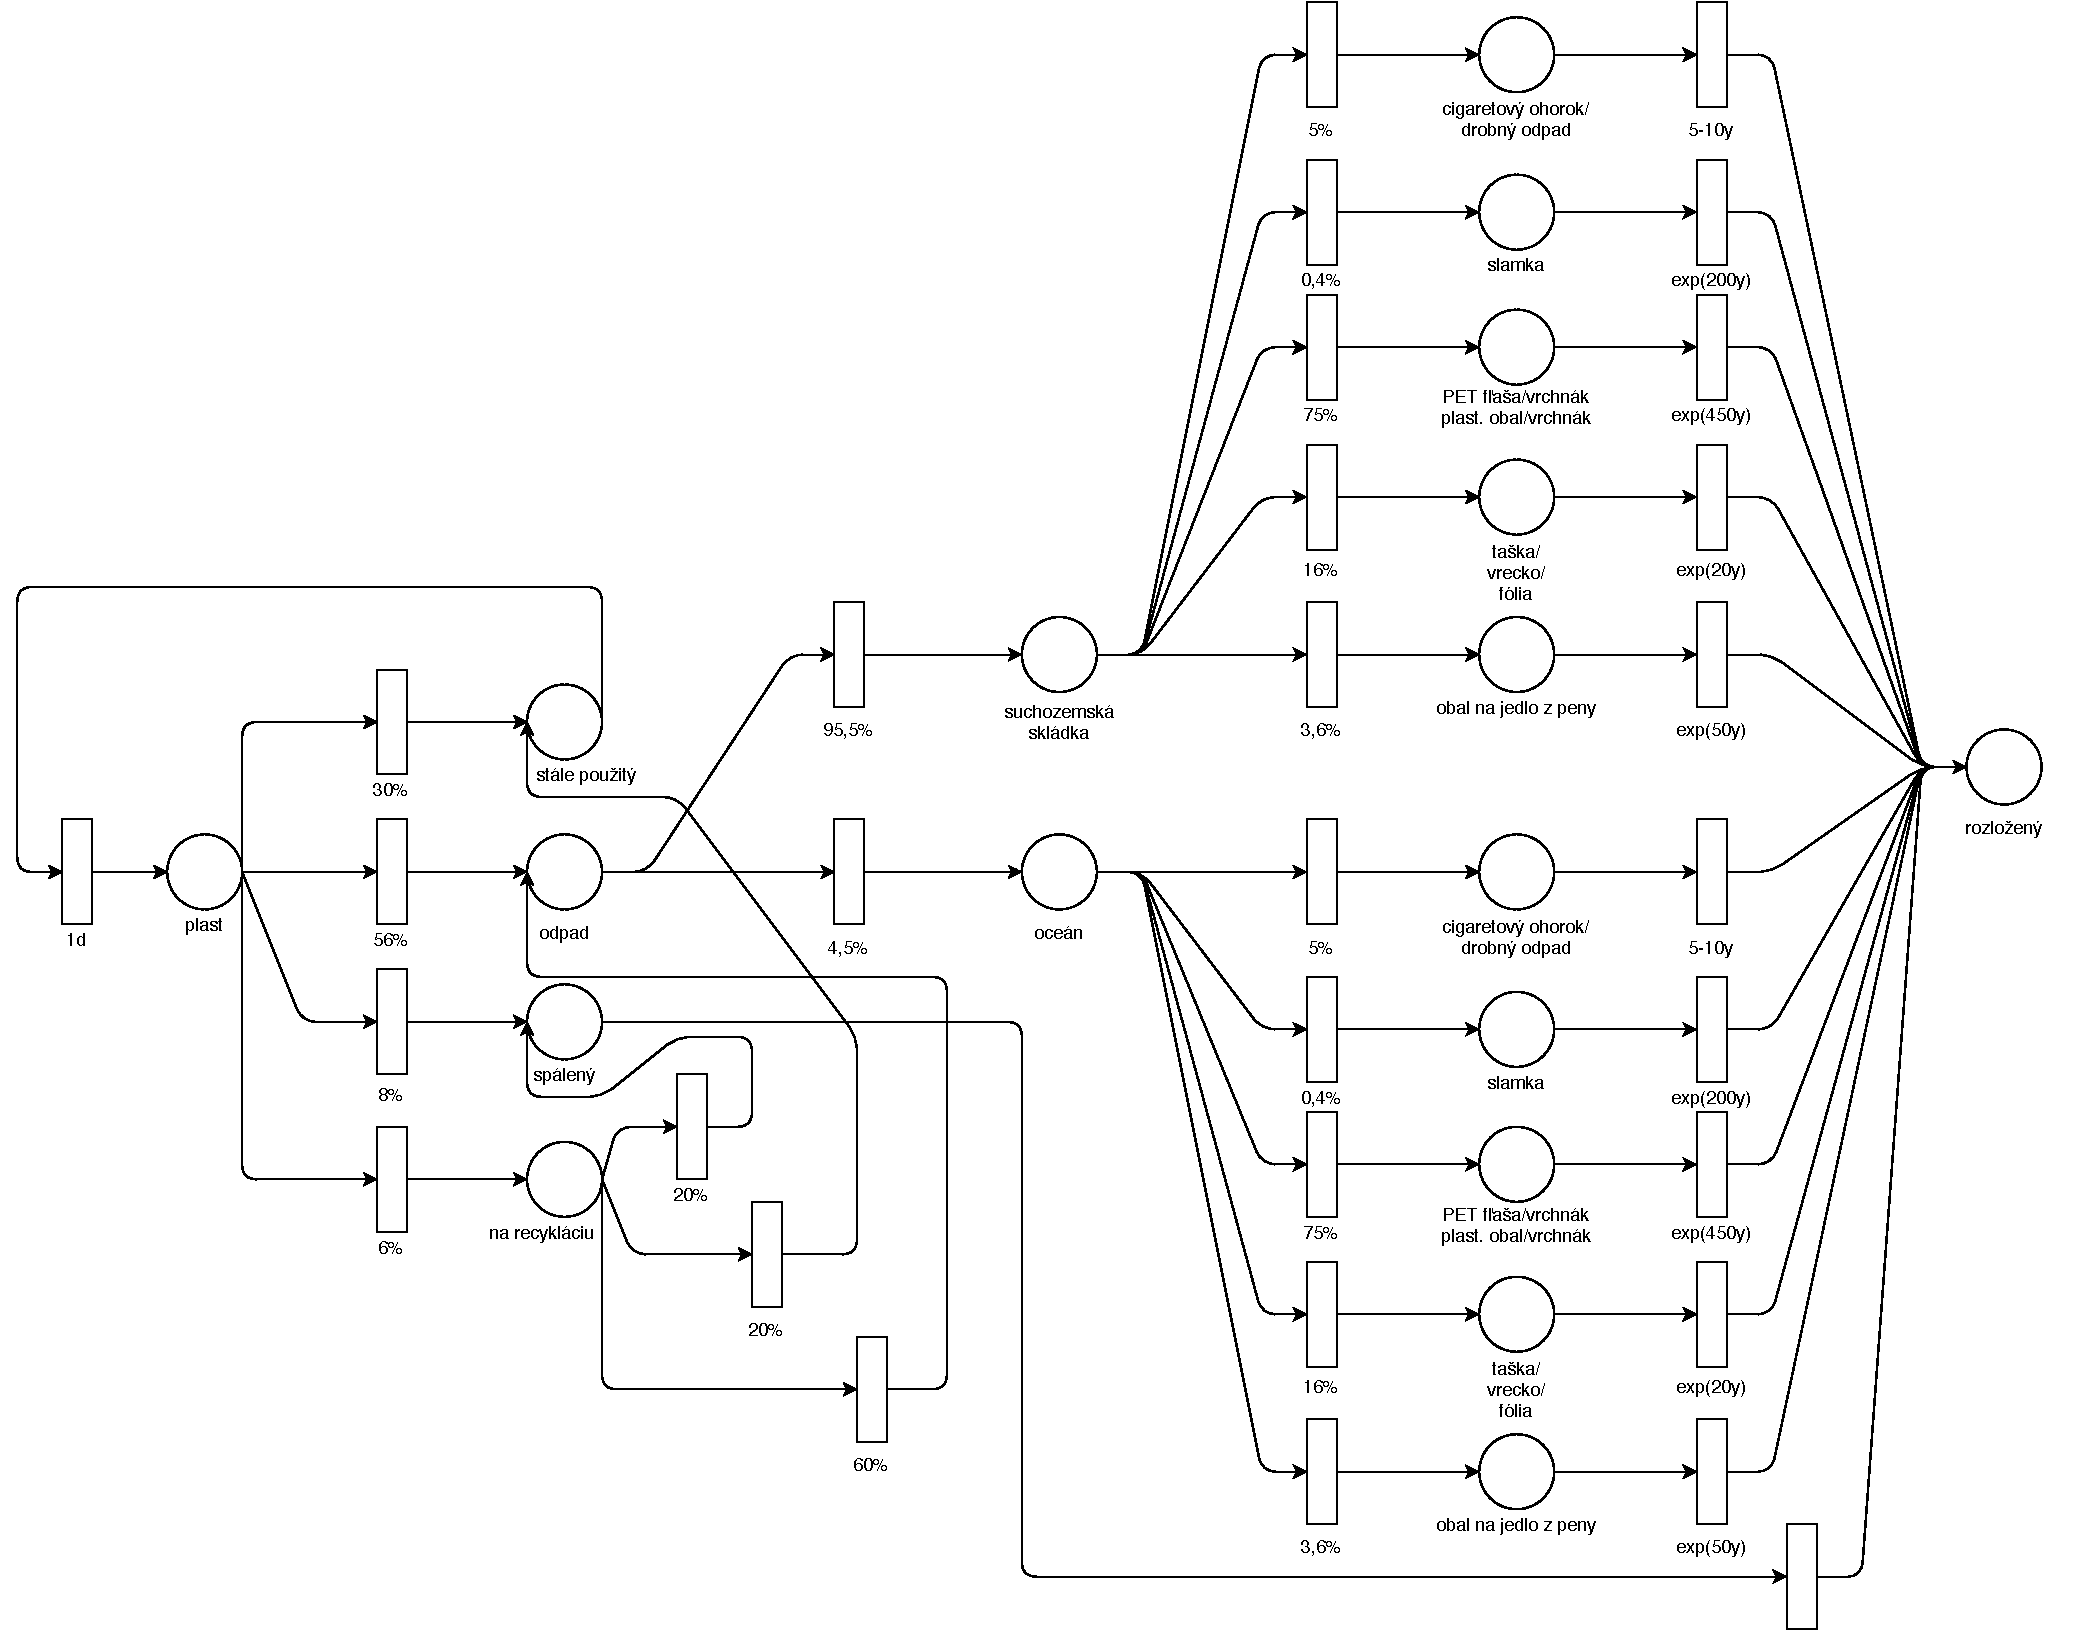
\includegraphics[width=1 \linewidth]{IMSpetri.pdf}
	\caption{Petriho sieť}
\end{figure}

\end{document}
